% Based on the supplied Brac University CSE400 final-year thesis template.
% Original abstract is copied byte-for-byte; see evidence_manifest.json.
\documentclass[12pt,oneside,openany]{report}
\usepackage[a4paper,width=150mm,top=25mm,bottom=25mm]{geometry}
\usepackage{fontspec}
\setmainfont{Times New Roman}
\newfontfamily\banglafont{Kohinoor Bangla}[Script=Bengali]
\newcommand{\bn}[1]{{\banglafont #1}}
\usepackage[english]{babel}
\usepackage{amsmath,amssymb,graphicx,booktabs,longtable,tabularx,array}
\usepackage{caption,float,tikz,enumitem,setspace,cite}
\usetikzlibrary{arrows.meta,positioning,shapes.geometric}
\usepackage[hyphens]{url}
\usepackage[colorlinks=true,allcolors=black]{hyperref}
\usepackage[nottoc]{tocbibind}
\setlength{\parindent}{0pt}
\setlength{\parskip}{6pt}
\setlength{\emergencystretch}{3em}
\renewcommand{\tabularxcolumn}[1]{>{\raggedright\arraybackslash}p{#1}}
\setlist{nosep,leftmargin=*}
\onehalfspacing
\newcommand{\code}[1]{\texttt{\small\detokenize{#1}}}
\newcommand{\pending}[1]{\textbf{Completion requirement:} #1}
\begin{document}
\hypersetup{pageanchor=false}
\begin{titlepage}\begin{center}
\vspace*{12mm}
{\fontsize{16}{21}\selectfont\bfseries Civic.ai - A Citizen Centric AI-Powered Government Service Assistant\par}
\vspace{12mm}by\par\vspace{6mm}
G.Araf Ahmed\\22101532\\
Mohammad Zunaid\\24241264\\
Md Shihab Sarker\\22101516\\
Fahim Foysal Abir\\22101543\\
Tapu Mohammad Fahad\\24241263
\vspace{12mm}

A thesis submitted to the Department of Computer Science and Engineering
in partial fulfillment of the requirements for the degree of
B.Sc. in Computer Science and Engineering
\vfill
Department of Computer Science and Engineering\\Brac University
\vspace{5mm}

\textit{Final thesis working manuscript}\par
Evidence snapshot: 24 September 2026\\
Submission semester and approval details: awaiting author confirmation
\vspace{5mm}

\copyright\ 2026. Brac University. All rights reserved.
\end{center}\end{titlepage}

\pagenumbering{roman}
\hypersetup{pageanchor=true}
\chapter*{Declaration}\addcontentsline{toc}{chapter}{Declaration}
This manuscript is prepared for the authors' review and signature. The authors must confirm that the work submitted is their own, that external sources are appropriately acknowledged and that the final document complies with the university's academic-integrity and tool-disclosure requirements.

\textbf{Author confirmation and signatures}

\begin{tabularx}{\linewidth}{Xl}
Md Shihab Sarker (22101516) & \rule{40mm}{0.4pt}\\[7mm]
G.Araf Ahmed (22101532) & \rule{40mm}{0.4pt}\\[7mm]
Tapu Mohammad Fahad (24241263) & \rule{40mm}{0.4pt}\\[7mm]
Fahim Foysal Abir (22101543) & \rule{40mm}{0.4pt}\\[7mm]
Mohammad Zunaid (24241264) & \rule{40mm}{0.4pt}
\end{tabularx}
\clearpage
\chapter*{Approval}\addcontentsline{toc}{chapter}{Approval}
\textit{Administrative page pending completion by the authors and examining committee. No approval or acceptance is asserted in this working manuscript.}

Thesis: Civic.ai - A Citizen Centric AI-Powered Government Service Assistant.

Thesis ID: T2520877. Submission semester and examination date require confirmation; the previous submission contains inconsistent dates.
\vspace{8mm}

\begin{tabularx}{\linewidth}{p{45mm}X}
Supervisor & Name, designation and signature to be confirmed\\[12mm]
Co-supervisor, if applicable & Name, designation and signature to be confirmed\\[12mm]
Thesis coordinator & Name, designation and signature to be confirmed\\[12mm]
Head of department & Name, designation and signature to be confirmed
\end{tabularx}
\clearpage
\chapter*{Ethics Statement}\addcontentsline{toc}{chapter}{Ethics Statement}
This project develops an informational assistant from collected government-service documents and prepared text derivatives. It does not issue official decisions, authenticate identities, process payments or approve applications. Public availability is not treated as an automatic redistribution licence. Original documents, derived text and source links must retain appropriate provenance and usage restrictions.

The manuscript includes an aggregate analysis of the team's needs-analysis questionnaire. The analysis excludes explicit non-consent and restricts substantive reporting to respondents who declared an adult age group; responses from minors and those with missing age are held out pending clarification of consent arrangements. Raw records and free-text responses are not included in the public thesis bundle. No ethics-board approval, representative population survey, completed chatbot usability study or independently adjudicated expert benchmark is claimed. Informal developer and domain-informed observations remain distinct from systematic human evaluation. Personal identification numbers, scans and private application records are not needed for the reported fixed-question experiments and should not be collected by a public deployment without appropriate safeguards.

The project used AI-assisted coding, debugging and manuscript preparation. The authors remain responsible for reviewing the implementation, references, analysis and final submission. Model-generated answers and automatic judges are not authoritative interpretations of government rules. Review flags and incomplete outputs are disclosed rather than represented as verified advice.
\clearpage

\phantomsection\addcontentsline{toc}{chapter}{Abstract}
\section*{Abstract}

Accessing government services in Bangladesh is often difficult due to confusing procedures, lack of clear and centralized information and reliance on middlemen. This prevents many citizens from accessing these services efficiently, resulting in unnecessary time delays and financial burdens. This thesis aims to solve this problem by developing an AI-Powered interactive system that provides citizen centric guidance for certain government services which will act as a digital bridge between citizens and government services. This system will inform users about required procedures and credentials of the respective services by offering dialogue and question-answering sessions. The outcome is a user-friendly, accessible system that empowers citizens with correct information, reduces dependency on intermediaries and simplifies interactions with government offices.

\vspace{1cm}
\textbf{Keywords:} Artificial Intelligence (AI), Government Services, Intermediaries, AI-Powered interactive system, Citizen centric guidance, Digital bridge, Dialogue and question-answering sessions, User-friendly and accessible system.
\pagebreak
\chapter*{Acknowledgement}\addcontentsline{toc}{chapter}{Acknowledgement}
We acknowledge the guidance provided during the thesis process and the public institutions whose service documents informed the knowledge corpus. We also acknowledge the developers of the open-source retrieval, embedding and local language-model software used in the implementation. Individual acknowledgements will be confirmed by the authors before submission.
\tableofcontents
\listoffigures
\listoftables
\chapter*{Nomenclature}\addcontentsline{toc}{chapter}{Nomenclature}
\begin{tabularx}{\linewidth}{lX}
BDRIS & Birth and Death Registration Information System\\
BRTA & Bangladesh Road Transport Authority\\
BM25 & Best Matching 25 lexical ranking method\\
LLM & Large language model\\
MRP & Machine-readable passport\\
NFC & Unicode Normalization Form C\\
OCR & Optical character recognition\\
QA & Question answering\\
RAG & Retrieval-augmented generation\\
RRF & Reciprocal rank fusion\\
\end{tabularx}
\clearpage\pagenumbering{arabic}
\chapter{Introduction}\section{Background}
Obtaining information about a government service often involves more than finding a website. A citizen must identify the correct procedure, understand the required documents and determine which conditions apply to their situation. In the Bangladeshi materials collected for this project, information is distributed across frequently asked questions, citizen charters, application instructions, fee tables and legal documents. Birth registration, passport applications and driving licences illustrate this difficulty: similar words can refer to different stages of a service.

This creates a gap between how information is published and how citizens ask for it. A document may organize requirements by legal provision, while a user asks a short question in everyday Bangla. Keyword search helps locate exact terms, but wording differences can obscure a relevant passage. Conversely, a result containing the right service name may describe the wrong procedure. Instructions for collecting a passport do not necessarily answer a question about applying for one.

Large language models (LLMs) offer a conversational way to explain information. However, an answer generated from model parameters alone need not reflect the supplied government documents or preserve their conditions. Retrieval-Augmented Generation (RAG) addresses this problem by supplying external passages during generation \cite{lewis2020rag}. Source-grounded retrieval makes the evidence inspectable and permits knowledge updates separately from model training. It improves the basis for answering, without guaranteeing that every retrieved passage or generated statement is correct.

In this context, we developed \textit{Civic.ai -- A Citizen-Centric AI-Powered Government Service Assistant}. Its implemented pipeline, referred to as CivicRAG, connects a predominantly Bangla civic-service corpus to a local question-answering interface. The current knowledge base covers birth and death registration, passport services and Bangladesh Road Transport Authority (BRTA) services. Civic.ai provides document-based guidance; it does not submit applications, access personal government records or replace the responsible authority.

\section{Rational of the Study or Motivation}
Our motivation combines an information-access need with a data-engineering problem. Citizens need understandable explanations, whereas published service information must first be collected and organized before a retrieval system can use it. Preparing this knowledge resource is a central contribution of the project.

The team's needs-analysis questionnaire supports this direction. Among valid responses from consenting adults, 55 of 77 submissions (71.4\%) indicated willingness to use the described AI assistant instead of an intermediary. Required-document guidance was selected by 62 of 77 (80.5\%), and payment or appointment information by 58 of 77 (75.3\%). These findings motivated our emphasis on requirements, procedures and source-traceable guidance. They describe interest in a prospective service, not measured adoption of Civic.ai.

Trust also influenced the design. Even under the questionnaire's hypothetical verified-information condition, 42 of 76 respondents (55.3\%) would recheck an answer. Therefore, the interface exposes evidence and available source links rather than asking users to rely on a response alone. Chapter 4 explains the survey processing and item-specific denominators; the detailed findings belong to the results chapter.

We selected local inference to support experimentation without sending each question and its evidence to a hosted generation service. This creates a trade-off between accessible deployment and response time. We consequently emphasize a manageable three-domain scope, reusable evaluation records and clear evidence boundaries rather than attempting every government service at once.

\section{Problem Statement}
The problem addressed by this thesis is how to turn heterogeneous civic-service documents into a usable, source-traceable Bangla question-answering system. The difficulty begins with the data: headings, conditions, tables and provenance can be lost during conversion or chunking. If these relationships are broken, later retrieval cannot reliably recover the intended meaning.

The next difficulty is applicability. A useful result must concern both the service and the action requested by the user. Finally, the generator must express that evidence correctly: it may otherwise omit a condition, combine unrelated requirements or return an incomplete answer. These stages are connected, but require separate examination.

We therefore investigate three questions:
\begin{enumerate}
\item How can collected materials become reusable domain-specific evidence units while preserving source relationships and unresolved quality issues?
\item How does CivicRAG's hybrid retrieval and evidence-selection configuration compare with a dense-only Simple RAG baseline under matched generation conditions?
\item How can retrieval behaviour and answer quality be evaluated separately to identify the strengths and limitations of the implemented system?
\end{enumerate}

\section{Objective}
Our \textbf{research objectives} are to develop and document the three-domain civic-service dataset, examine the selected RAG configuration against a matched baseline, and analyse retrieval and generation using reproducible evidence. Dataset preparation and representation are described in Chapter 4; comparative observations and evaluation limitations are addressed in Chapter 5.

Our \textbf{system objectives} are to support Bangla questions within a selected service domain, retrieve evidence through semantic and lexical matching, generate a Bangla explanation from the supplied material, and retain the passages and identifiers needed to inspect a response. Additional engineering objectives are local execution, configurable models and reversible changes through version control. These objectives inform the requirements in Chapter 3.

The study adapts established RAG techniques rather than introducing a new foundation model. Indexing documents is knowledge-base construction, not model training. The intended contribution is a developed and evaluated civic-service system supported by a traceable dataset, with claims limited to implemented functions and recorded experiments.

\section{Methodology in Brief }
The methodology separates offline preparation from online answering. Offline, original materials are preserved, prepared text is normalized, and document-aware chunks receive identifiers and metadata. Each chunk retains searchable text and source evidence. BGE-M3 embeds the searchable representation \cite{bgem3}; ChromaDB stores vectors and linked text \cite{chroma}. A separate BM25 index supports lexical retrieval.

Online, the question is normalized and searched within the selected domain. Dense and BM25 rankings are combined using weighted Reciprocal Rank Fusion (RRF), followed by reranking and automatic applicability-based evidence selection. Selected passages are passed to a local generator through Ollama \cite{ollama}. The main paired comparison uses Qwen3:8b \cite{qwen3}, with checks for unsuitable-language output and incomplete generation.

The modular pipeline permits independent inspection of preparation, retrieval and generation. Saved questions, contexts, answers and configuration records support evaluation without repeatedly generating answers. A matched dense-only baseline provides the system comparison, while retrieval-only experiments examine ranked passages separately.

\section{Scopes and Challenges}
\textbf{Current scope.} Civic.ai handles single-turn informational questions using three domain-specific collections. Sources contain Bangla, English and mixed-language content, but the principal interface and comparison target Bangla questions and Bangla responses. The 30-question comparison contains ten passport, ten birth-registration and ten driving-licence questions. Death registration and other BRTA services exist in the corpus but have no dedicated questions in this comparison.

\textbf{Data challenges.} Uneven formatting, scanned text, missing URLs and historical instructions complicate preparation. We retain provenance and review flags rather than treating every converted document as independently verified.

\textbf{Retrieval challenges.} Different procedures share vocabulary, and broad questions can require several sections. Domain selection reduces cross-service interference, but relevance and coverage still require evaluation.

\textbf{Generation challenges.} Local models may omit conditions, combine incompatible evidence or use unnatural Bangla. Output limits can interrupt long checklists. Direct, paraphrased and scenario-based questions use the same pipeline, although the main set does not establish robustness across all these variants.

\textbf{Future expansion.} Additional domains, more varied unseen questions and stronger hardware are possible extensions. Transaction execution, document authentication and live application-status lookup remain outside the implementation. Reused development questions support a bounded comparison, not unrestricted performance claims.

\section{Team Overview}
The project team consists of Md Shihab Sarker, G.Araf Ahmed, Tapu Mohammad Fahad, Fahim Foysal Abir and Mohammad Zunaid. Our work brings together source collection, machine-readable document preparation, pipeline development, experimental review and thesis documentation. These activities are interdependent: preparation changes can affect retrieval, while answer failures can expose missing conditions in evidence.

Source directories, experiment records and Git history keep the outputs traceable. They are used to document the project rather than infer individual responsibilities or hours worked from filenames. Section 3.6 describes the completed development sequence and its controls.

\section{Key Learnings and Insights}
The principal architectural lesson is that finding a related document and answering the question are different tasks. Combining retrieval methods creates opportunities to find evidence, but additional passages can introduce distractions. Selection therefore needs to preserve service conditions rather than simply increase the amount of context.

Dataset development demonstrated the value of original-file preservation, headings and stable identifiers. Bangla processing showed that encoding consistency is necessary but insufficient: normalized text may still contain OCR errors or ambiguous wording. Both structure and language quality affect downstream behaviour.

Finally, evaluation must distinguish retrieval quality, answer support and usefulness. Source IDs make an answer inspectable, but do not prove each statement. A longer response may cover more cases without being more precise. These lessons shape the requirements and methodology in the following chapters.

\chapter{Literature Review}\section{Preliminaries}
\subsection{Retrieval-Augmented Generation}
RAG combines an external retrieval mechanism with a generator \cite{lewis2020rag}. In this implementation, retrieval selects passages at inference time and passes them to a pretrained model. No joint retriever-generator training is performed. This distinction matters because updating the corpus changes available evidence, but not the model's learned ability to reason about that evidence.

\subsection{Dense Retrieval, Lexical Retrieval and Fusion}
Dense retrieval maps text to vectors and ranks candidate passages by vector proximity. BM25 instead ranks token overlap using term frequency and length normalization \cite{bm25}. The channels can complement one another: semantic matching may accommodate paraphrases, while token matching can preserve important form numbers and service names. Neither channel checks whether a legal provision remains in force.

RRF combines ordered result lists rather than directly adding incompatible raw scores \cite{rrf}. CivicRAG uses a weighted form. Fusion is a way to construct a hybrid result list, not the definition of hybrid retrieval itself: weighted score fusion would be another possible combination method. Its effectiveness must be tested rather than inferred from the presence of two retrievers.

\subsection{Reranking and Context Selection}
A cross-encoder scores a query and passage jointly, unlike independently encoded dense vectors. CivicRAG configures the multilingual BGE reranker \cite{bgereranker}. Applicability selection is a separate, project-specific rule layer. It uses section scope and service/action vocabulary to remove or reorder passages. A reranker relevance score and a selector decision are neither probabilities of truth nor substitutes for claim-level validation.

\section{Review of Existing Research}
\subsection{NextRAG: Principal Architectural Inspiration}
NextRAG addresses bilingual financial QA from Bangladeshi documents. Its method combines dense retrieval, BM25 and Dirichlet-smoothed query-likelihood retrieval, followed by weighted RRF, reranking and language-aware generation. Its reported evaluation includes reference-answer cosine similarity, F1 and inference time \cite{nextrag}. The shared document-language setting motivates borrowing retrieval components, but financial and civic-service applicability are not equivalent tasks.

\begin{table}[htbp]\centering\small
\caption{Relationship between NextRAG and the implemented CivicRAG configuration.}
\begin{tabularx}{\linewidth}{p{30mm}XX}\toprule
Aspect & NextRAG & CivicRAG\\\midrule
Application & Financial information & Three civic-service domains\\
Retrieval & Dense, BM25, Dirichlet QLM & Dense and BM25\\
Combination & Weighted RRF & Weighted RRF, two channels\\
Post-retrieval & Reranking & Reranking and heuristic applicability selection\\
Evidence preparation & Financial document processing & Typed evidence, source register and dual text representations\\
Reported comparison & Bilingual reference-answer evaluation & Paired Bangla development questions; saved outputs and diagnostic analysis\\
Generator identity & Includes Llama 3.1 8B & Main comparison Qwen3:8b; local llama3 is not Llama 3.1\\\bottomrule
\end{tabularx}\end{table}

This relationship is described as inspiration rather than replication. CivicRAG does not implement the third Dirichlet channel or reproduce the financial benchmark. The paper's numerical results are not used as baselines for our different corpus and question set. Its reference-answer metrics are also not replaced by unlabelled similarity between two model outputs.

\subsection{Multilingual Embeddings and Local Generators}
BGE-M3 supports multilingual text representation and multiple retrieval modes \cite{bgem3}. CivicRAG uses its dense embeddings only; its sparse branch is separately implemented BM25, not BGE-M3's learned sparse mode. This clarification prevents the embedding model's full capabilities from being mistaken for implemented functionality.

Qwen3 supplies thinking and non-thinking modes in the same model family \cite{qwen3}. The selected local deployment uses the non-thinking mode for the recorded main comparison. This is an inference setting, not evidence that reasoning would improve or reduce civic-answer quality. No controlled thinking-mode ablation was completed. Qwen2.5 and Llama 3 were also tested locally \cite{qwen25,llama3card}. These are specific deployed model variants, not interchangeable labels for their entire families.

\subsection{Context Distraction and Diagnostic Evaluation}
Research on long-context language models shows that access to relevant information does not guarantee its effective use, and that placement can affect performance \cite{lostmiddle}. The project's selected-evidence and evidence-order trials investigate a related practical issue: whether unrelated service passages change an otherwise useful answer. They are small generation-only diagnostics. They do not demonstrate that a manually chosen context can be selected automatically for arbitrary questions.

\subsection{Other Bangla RAG Approaches}
TraSe investigates Bangla Wikipedia question answering using translative prompting and answer selection, with both automatic and human-in-the-loop retrieval \cite{trase}. Its distinction between automatically retrieved and human-selected contexts is useful for diagnosing our system: generation with manually selected evidence tests a different capability from end-to-end retrieval. CivicRAG's relevant-only trials follow this diagnostic logic, but do not implement TraSe's translation and answer-selection architecture. Their better outputs cannot be reported as automatic retrieval accuracy.

HybridRAG-BN is a recent preprint combining BM25 and BGE-M3 retrieval with generation and a fine-tuned verification stage \cite{hybridragbn}. Its use of verification highlights that retrieval relevance and answer correctness are separate problems. CivicRAG shares established retrieval components but does not train a verifier or implement that paper's web-assisted fallback. Its competition scores are not directly comparable with our civic-service questions. These approaches inform possible future experiments, rather than retrospectively becoming components of our implementation.

\subsection{Automatic RAG Evaluation}
RAGAS separates aspects of retrieval and generation quality through model-assisted metrics \cite{ragas}. Faithfulness checks whether response claims are supported by the supplied context. Response relevance concerns how well an answer addresses its question. A source-supported response can still answer the wrong task, so no single score is a comprehensive measure of factual correctness.

The implemented evaluator uses a local judge and documents its limitations. It does not have reviewed reference answers or gold relevance labels for the current 30 questions. Therefore reference semantic similarity, retrieval recall, MRR and nDCG are not reported for that experiment. Reusing metric names from an earlier submission without the necessary labels would be methodologically incorrect.

\section{Summary of Key Findings}
The literature motivates multilingual retrieval, complementary lexical matching, reranking and separate assessment of context and response. Our contribution lies in the civic corpus and its traceable operationalization, with an evaluated integration of established methods. Neither the evidence selector nor the local model is presented as a newly trained state-of-the-art method.

Only sources that can be tied to the implemented method or a specific discussion are retained. Earlier draft reference lists are not inherited wholesale. Related architectures mentioned during development but not implemented are not presented as components of CivicRAG. The main comparison tests the combined configuration against dense-only retrieval; it cannot isolate the causal effect of RRF, reranking or selection individually.

\chapter{Requirements, Impacts and Constraints}\section{Final Specifications and Requirements}
The functional requirements are domain-scoped retrieval, Bangla-oriented generation, inspectable evidence, model selection and persistent experiment records. The system must distinguish the search representation from answer evidence, expose the passages actually supplied to generation and preserve a rollback path for changes. These requirements are implemented through domain configurations, the source register, structured response fields and Git revisions.

\begin{table}[htbp]\centering\small
\caption{Implemented requirements and limits of verification.}
\begin{tabularx}{\linewidth}{p{36mm}XX}\toprule
Requirement & Implementation & Verification boundary\\\midrule
Domain selection & Separate configurations and Chroma collections & Does not guarantee all out-of-domain rejection\\
Evidence traceability & Chunk IDs, metadata, source paths and available URLs & Footer is not claim-level citation verification\\
Bangla response & Prompt and language safety check & Fluency and semantic accuracy remain imperfect\\
Local execution & Ollama generation; locally cached embeddings & Latency remains substantial\\
Reproducible comparison & Saved questions, answers, contexts and hashes & One run per configuration; reused questions\\
Reversible development & Git revisions and rollback tags & Untracked artifacts need explicit preservation\\\bottomrule
\end{tabularx}\end{table}

The selected comparison requests Qwen3 explicitly. Some configuration files retain Llama 3.2 as a default; this does not identify the model used in saved experiments. Execution records, not an isolated default value, determine the evaluated configuration. Similarly, the selected-evidence branch allows six passages even though the legacy generation configuration retains a three-passage setting.

\section{Societal Impact}
The intended benefit is easier access to structured explanations of civic procedures. Bangla responses and inspectable evidence may reduce the effort needed to navigate multiple files. However, the reported experiments involve questions and saved model outputs rather than a deployed population study. Improvements in accessibility, trust or intermediary dependence remain intended outcomes, not measured effects.

Incorrect fees or procedure instructions can create practical harm. The interface should therefore be understood as guidance to inspect alongside official sources. A source link gives a route for checking information, but some corpus records have missing URLs or unresolved original matches. The manuscript does not imply official endorsement or authoritative legal status.

\section{Environmental Impact}
Local inference uses electricity and hardware resources. The project reuses pretrained models rather than training a foundation model, but no power measurements or carbon accounting were performed. Response time is not a substitute for energy measurement. A future study would log power draw, duration and system utilization under comparable conditions before making environmental-efficiency claims.

\section{Ethical Issues}
Three ethical concerns guide the design. First, evidence may be outdated or inapplicable even when faithfully quoted. Second, local models can combine requirements from different categories. Third, a user may interpret a confident answer as official advice. The system exposes provenance and incomplete-output warnings, but these mechanisms do not eliminate those risks.

Data curation preserves original files and records derivation rather than silently overwriting sources. Automatically detected flags indicate unresolved checks, not conclusive judgments that a file is wrong. Human review remains necessary for conflicting fees, applicability dates and OCR-sensitive legal text. Informal user preference is recorded as an observation, not converted into an invented expert accuracy score.

\section{Standards and Interoperability}
The implementation uses UTF-8 text, Unicode NFC normalization, JSON/JSONL records and SHA-256 hashes. These choices support interoperable storage and change detection. They do not constitute certification under a government, security, accessibility or quality-management standard. No compliance audit is claimed.

The source and search representations retain machine-readable identifiers that permit reproducible joins across retrieval, evidence selection and evaluation. Documents without public URLs still retain local provenance; they must not be assigned fabricated URLs. Redistribution of original PDFs and personal information requires separate permission review.

\section{Project Management Plan}
The completed work proceeded through corpus preparation, a birth/death-registration implementation, extension to passport and BRTA, generation diagnostics and a matched baseline comparison. Later changes were preserved as candidates and Git revisions. The final evaluation configuration is identified through hashes rather than by describing every subsequent draft as active.

For finalization, architecture and corpus changes are separated from reporting. The outstanding automatic evaluation may finish without modifying the answer files. The thesis tables are regenerated from those artifacts, while the Abstract is checked against its immutable source. Changes that would require new answer generation are not silently included in the current comparison.

\section{Risk Management}
\begin{longtable}{p{34mm}p{49mm}p{54mm}}
\caption{Principal project risks and controls.}\label{tab:risks}\\\toprule
Risk & Existing control & Residual issue\\\midrule\endfirsthead
\toprule Risk & Existing control & Residual issue\\\midrule\endhead
Wrong procedure & Domain scope, reranking, applicability vocabulary & Similar headings and unclassified passages remain\\
Historical rules & Date fields and audit flags & Dates and legal applicability not independently verified\\
OCR corruption & Original-file links and review flags & Not all long legal documents manually checked\\
Context crowding & Whole-chunk budget and family-order fix & Broad queries may still require omitted evidence\\
Wrong generation & Evidence prompt and language check & No complete semantic entailment guard\\
Truncation & Finish-reason warning & Warning does not complete an interrupted answer\\
Evaluation bias & Matched inputs and disclosed development set & Reuse, self-judging and small sample remain\\
Version confusion & Hash manifests and rollback revisions & Index rebuilds and deployment must respect the manifest\\\bottomrule
\end{longtable}

\section{Economic Analysis}
The main generation runs use local Ollama rather than paid per-request inference. This establishes the absence of such API charges for those runs, not a zero-cost system. Hardware ownership, electricity, source preparation and review time remain costs. No invoices, time sheets or power logs support a complete monetary analysis, so no fabricated budget or savings figure is included.

At the recorded mean latency, a sequential 30-question run takes substantial wall-clock time. This limits the practicality of repeated full-batch experiments on the available machine and motivates reusing saved outputs for evaluation. Latency reduction through different hardware or smaller contexts is a future optimization, not a demonstrated economic benefit.

\chapter{Proposed Methodology}\section{Design Process or Methodology Overview }
CivicRAG separates offline corpus/index construction from online retrieval and answer generation. The pipeline diagram in Figure~\ref{fig:architecture} describes the selected-evidence configuration used by the main CivicRAG run. Legacy controlled-answer branches remain in the repository for rollback but are not the answer route of this comparison.

\begin{figure}[p]\centering
\begin{singlespace}
\begin{tikzpicture}[x=1cm,y=1cm]
\tikzset{civicbox/.append style={font=\footnotesize,inner sep=2mm}}
\fill[rounded corners=3mm,civicTeal!4] (-0.2,0.9) rectangle (14.2,-4.1);
\node[anchor=west,font=\small\bfseries,text=civicTeal] at (0,0.55) {OFFLINE: CORPUS AND INDEX PREPARATION};
\node[civicbox,text width=5.5cm] (raw) at (3.1,-0.45) {Source files + prepared text\\PDF / DOCX / HTML / JSON};
\node[civicbox,text width=5.5cm] (chunk) at (10.6,-0.45) {Normalize and create typed chunks\\Attach IDs and provenance};
\draw[civicarr] (raw)--(chunk);
\node[civicbox,text width=12.6cm] (represent) at (7,-1.85) {Linked representations per chunk: search text $r_i$ and evidence $e_i$\\Only $r_i$ is embedded; $e_i$ is preserved as source content};
\draw[civicarr] (chunk.south)--(represent.north -| chunk.south);
\node[civicbox,text width=12.6cm] (indexes) at (7,-3.2) {BGE-M3($r_i$) $\rightarrow$ Chroma dense index\quad |\quad BM25 tokens from $r_i$\\Evidence and metadata remain linked by the same chunk ID};
\draw[civicarr] (represent)--(indexes);

\fill[rounded corners=3mm,civicBlue!4] (-0.2,-4.5) rectangle (14.2,-16.95);
\node[anchor=west,font=\small\bfseries,text=civicBlue] at (0,-4.9) {ONLINE: SHARED THREE-DOMAIN QUESTION ANSWERING};
\node[civicbox,text width=11.6cm] (query) at (7,-5.8) {Bangla question + selected domain\\Birth/death registration / Passport / BRTA};
\node[civicbox,text width=5.3cm] (dense) at (3.3,-7.25) {Dense search: top 20\\BGE-M3 query vector + Chroma};
\node[civicbox,text width=5.3cm] (sparse) at (10.7,-7.25) {BM25 search: top 20\\Query tokens + sparse index};
\draw[civicarr] (query.south)--++(0,-0.25)-|(dense.north);
\draw[civicarr] (query.south)--++(0,-0.25)-|(sparse.north);
\draw[civicarr,dashed] (indexes.west)--(-0.05,-3.2)--(-0.05,-7.25)--(dense.west);
\draw[civicarr,dashed] (indexes.east)--(14.05,-3.2)--(14.05,-7.25)--(sparse.east);
\node[civicbox,text width=11.6cm] (rrf) at (7,-8.75) {Weighted RRF: merge ranks, retain up to 15 candidates};
\draw[civicarr] (dense.south)--++(0,-0.25)-|(rrf.north);
\draw[civicarr] (sparse.south)--++(0,-0.25)-|(rrf.north);
\node[civicbox,text width=11.6cm] (rank) at (7,-10.0) {BGE cross-encoder reranking: ALL domains\\Lexical fallback if the cross-encoder is unavailable};
\draw[civicarr] (rrf)--(rank);
\node[civicbox,draw=civicGold,fill=civicGold!8,text width=11.6cm] (rules) at (7,-11.5) {Conditional birth-registration rules only:\\score adjustments and correction-fee supplementation\\Passport / BRTA skip these extra rules, not reranking};
\draw[civicarr] (rank)--(rules);
\node[civicbox,text width=11.6cm] (select) at (7,-13.1) {Shared applicability selector + compatible-family ordering\\Original evidence by ID; at most 6 chunks / 14,000 characters};
\draw[civicarr] (rules)--(select);
\node[civicbox,text width=11.6cm] (llm) at (7,-14.6) {Qwen3:8b: question + selected source evidence\\No evidence: clarification instead of an LLM answer};
\draw[civicarr] (select)--(llm);
\node[civicbox,text width=11.6cm] (answer) at (7,-16.1) {Bangla response + supplied source IDs\\Language check and incomplete-output warning};
\draw[civicarr] (llm)--(answer);
\end{tikzpicture}
\end{singlespace}
\caption{Earlier compact CivicRAG architecture with offline/online organization for three domains. Dashed arrows indicate index access. The gold box distinguishes domain-specific rules from shared reranking. The selected-evidence route bypasses the legacy controlled-answer branch.}\label{fig:architecture}
\end{figure}


The diagram retains the P2 separation between offline preparation and online answering, but explicitly connects stored evidence to generation and distinguishes shared components from conditional rules. The upper stage constructs retrieval resources; it is indexing, not LLM training. The lower stage searches and selects evidence before generating text. Dense retrieval, BM25, rank fusion, cross-encoder reranking, applicability selection and local generation are shared across all three configured domains. Only the additional registration-specific adjustments are conditional on the birth/death domain.

\section{Preliminary Design or Design (Model) Specification}
The P2 design emphasized birth/death registration, hybrid retrieval and controlled answer paths. Later work extended the corpus to passport and BRTA, added applicability selection and changed the main generator comparison to Qwen3. The final reported route therefore differs from the old diagrams that send every answer through a generic safe-path box.

The system is not an autonomous agent that performs government actions. Its task is single-turn retrieval and evidence-conditioned text generation. A domain is selected before retrieval. A targeted cross-domain aggregate guard handles certain multi-service questions, but comprehensive intent recognition is not claimed. Neither the lexical rules nor the selector is a separately trained classifier.

The implemented alternatives are the matched dense-only baseline and the design using hybrid retrieval, reranking and selected evidence. Both have saved 30-question executions. The relevant-only and evidence-order diagnostics isolate context handling but do not simulate a complete deployment. Their outputs verify specific design behaviours; a selector-off ablation remains unexecuted. Controlled settings appear in Section 4.4 and observed outcomes in Chapter 5.

\pending{Task DS-01: if component-level verification is required, freeze both configurations and run a selector-off comparison on the same questions, saving contexts, answers, timings and routes. Do not describe it as completed before its artifacts exist. The existing paired design comparison can be reported without inventing a simulation.}

\section{Data Collection -(If
Applicable)}
\paragraph{Needs-Analysis Questionnaire.}
The team supplied three CSV questionnaire exports, each containing 46 columns. They cover demographics, experiences with birth registration, passport and BRTA services, and a common nine-item block concerning a prospective AI assistant. The three versions place the service-specific blocks in different orders. Analysis aligns those blocks before checking identical submissions and uses column positions because several free-response headers repeat. The survey is a requirements input, not additional retrieval evidence, and is not ingested into the chatbot's knowledge base.

Only affirmative-consent records with a declared adult age group enter the main descriptive analysis. This conservative inclusion rule was applied when preparing the thesis analysis; it is not claimed to have been preregistered. Missing responses are excluded separately for each item, not interpreted as rejection. Percentages are computed as $100c/n_v$, where $c$ is the number selecting a response and $n_v$ the number answering that item. Multiple-selection items count each explicitly selected option once per submission, so their percentages need not sum to 100. A free-text ``all options'' response is retained in the denominator but not expanded into checked options. Open-text answers are not quoted publicly or automatically coded as validated themes.

The exported consent field establishes an affirmative response, not independent ethics approval. Recruitment method, invitation count, repeat-participation controls and consent arrangements for minors were not supplied. Accordingly, a response rate and nationally representative estimates cannot be calculated. The BRTA website question also combines a Bangladesh address with \code{rsta.gov.bt}; that item is not used to claim verified BRTA website usage. The main findings use the identically positioned common AI block and are reported in Chapter 5.

\paragraph{Source Families and Original Preservation.}
The birth/death collection contains structured JSON and prepared Markdown derived from FAQs, laws, rules, fees, correction processes and application guidance. Passport and BRTA were supplied as original-file directories and separately prepared Markdown. Passport derivatives are registered from \code{cleaned_md}; BRTA derivatives from \code{brta} and \code{fahim_brta}. Directories explicitly marked original are reference materials, not duplicate text automatically added to the answer corpus.

The register preserves document IDs, relative paths, snapshots, hashes, candidate original-file matches, inclusion history and chunk IDs. Candidate original matches do not certify textual fidelity. Some matches remain unresolved and are flagged. The distinction between collected originals and derivatives avoids counting the same information twice as independent evidence.

The corpus is a retrieval resource, not a newly annotated gold-answer benchmark. Its novelty is the organization of selected civic-service material into a source-traceable, machine-usable representation spanning the three domains. It is neither a census of all government documents nor a guarantee of current legal validity.

\subsection{Data Cleaning}
\begin{figure}[htbp]\centering
\begin{singlespace}
\begin{tikzpicture}[node distance=7mm]
\node[civicbox,text width=12.3cm] (original) {Collected originals + team-prepared derivatives\\Preserve originals; record the source relationship};
\node[civicbox,text width=12.3cm,below=of original] (parse) {Parse Markdown / structured JSON; read available front matter\\Normalize Unicode NFC and remove selected authoring artifacts};
\node[civicbox,text width=12.3cm,below=of parse] (split) {Document-type / heading-aware chunking\\Preserve FAQ pairs, fee conditions and procedure sections where available};
\node[civicbox,text width=12.3cm,below=of split] (meta) {Attach chunk IDs, document types, headings, source paths and available URLs\\Retain unresolved provenance / OCR / applicability flags};
\node[civicbox,text width=12.3cm,below=of meta] (output) {Domain JSONL: $(\mathrm{id}_i,r_i,e_i,m_i)$\\Build indexes from the configured active corpus};
\foreach \a/\b in {original/parse,parse/split,split/meta,meta/output}{\draw[civicarr] (\a)--(\b);}
\end{tikzpicture}
\end{singlespace}
\caption{Source-preserving preparation of the active corpus: original materials remain available while normalized derivatives are organized into identifiable retrieval units. Separate cleanup candidates are not substituted for the evaluated corpus.}\label{fig:preprocessing}
\end{figure}

Figure~\ref{fig:preprocessing} separates preservation of original materials from transformations applied to the machine-readable derivatives. The archived P2 diagram is a design reference; this final diagram describes supported preparation steps rather than assuming every originally illustrated operation was automated.

The active passport/BRTA ingestion parses simple front matter, normalizes NFC text, removes explicit authoring citation markers and selected invisible characters, and tracks headings. It preserves malformed or unrecognized material instead of making broad deletions. The work does not substantiate a universal automatic OCR repair or Bijoy-to-Unicode conversion stage for every supplied file; such claims from illustrative diagrams are not carried forward.

Separate cleanup candidates remove recognized authoring preambles and boilerplate and preserve larger structural units. Their manifests record changes and review flags. Those candidates must be distinguished from the evaluated corpus. At the audited snapshot, the active domain configurations still reference the heading-aware v2 passport/BRTA files. A later cleanup directory alone is not evidence that its contents were activated in ChromaDB or used in the saved answers.

\subsection{Data Transformation}
Document-type-aware transformation retains question-answer pairs, headings, fee rows and process sections where the source permits. A chunk should keep its governing condition with its answer. Splitting a heading from its body can make retrieval apparently relevant while the actual content answers a different question. Heading-aware ingestion was introduced to reduce this failure, but long unstructured legal OCR remains difficult.

Each chunk has the form
\begin{equation}
c_i=(\mathrm{id}_i,r_i,e_i,m_i),
\end{equation}
where $e_i$ is evidence content, $r_i$ is search text and $m_i$ is metadata. Search text may include aliases or section descriptors. These additions help search; they are not source facts and are not meant to become answer evidence. No query-specific reference answer is inserted into the generator merely because it resembles a test question.

\subsection{Data Integration}
\begin{figure}[htbp]\centering
\begin{singlespace}
\begin{tikzpicture}[x=1cm,y=1cm]
\tikzset{civicbox/.append style={font=\footnotesize,inner sep=2mm}}
\node[civicbox,text width=12cm] (record) at (7,0) {One chunk record: $c_i=(\mathrm{id}_i,r_i,e_i,m_i)$};
\node[civicbox,text width=3.5cm] (search) at (2.1,-1.7) {Search text $r_i$\\Aliases / search wording};
\node[civicbox,text width=3.5cm] (evidence) at (7,-1.7) {Evidence $e_i$\\Original source content};
\node[civicbox,text width=3.5cm] (metadata) at (11.9,-1.7) {Metadata $m_i$\\Type, heading, source};
\draw[civicarr] (record.south)--++(0,-0.25)-|(search.north);
\draw[civicarr] (record)--(evidence);
\draw[civicarr] (record.south)--++(0,-0.25)-|(metadata.north);
\node[civicbox,text width=3.5cm] (embed) at (2.1,-3.4) {BGE-M3 encoder\\Dense vector $v_i$};
\draw[civicarr] (search)--(embed);
\node[civicbox,text width=12cm] (storage) at (7,-5.05) {Chroma record: ID + vector $v_i$ + document $e_i$ + metadata $m_i$\\Active JSONL also retains the complete chunk record};
\draw[civicarr] (embed.south)--++(0,-0.3)-|(storage.north);
\draw[civicarr] (evidence)--(storage);
\draw[civicarr] (metadata.south)--++(0,-1.1)-|(storage.north east);
\node[civicbox,text width=12cm] (fetch) at (7,-6.7) {Dense search returns matching IDs\\Runtime looks up those IDs in the active JSONL chunk map};
\draw[civicarr] (storage)--(fetch);
\node[civicbox,text width=12cm] (generation) at (7,-8.35) {Selector retains applicable evidence $e_i$\\LLM receives the question and text, not vector coordinates};
\draw[civicarr] (fetch)--(generation);
\end{tikzpicture}
\end{singlespace}
\caption{How answer evidence remains connected to a vector without being generated by the database. BM25 is a separate index of $r_i$, omitted here to isolate the dense-storage link. All arrows entering storage denote stored fields, not additional embeddings.}\label{fig:evidence-linkage}
\end{figure}

Each domain has its own configured JSONL corpus and Chroma collection. Metadata preserves service context and available source URLs. A stable chunk ID joins vector results back to the source record. The runtime dense retriever obtains IDs from Chroma and reconstructs retrieval results from the in-memory chunk map, making the active JSONL and index consistency essential.

In \code{scripts/build_index.py}, embeddings are computed from \code{retrieval_text}, whereas Chroma's \code{documents} contain \code{content}. The versioned ingestion script follows the same storage separation. Therefore answer evidence is stored alongside a vector; it is not itself an answer produced by Chroma. Chroma is a retrieval store, and the LLM produces the response only after evidence selection.

Figure~\ref{fig:evidence-linkage} makes this relationship explicit. If $I_q$ is a list of retrieved chunk IDs and $M$ is the active chunk map, then the corresponding evidence is obtained by
\begin{equation}
E_q=[M[i].\mathrm{content}:i\in I_q].
\end{equation}
This is an identifier lookup, not a comparison between a database-generated answer and a reference answer. The subsequent selector can remove candidates or append compatible family members; therefore the final supplied evidence need not equal the first retrieved list.

\subsection{Data Reduction }
Reduction is treated conservatively. FAQ duplicate handling and chunk boundaries can reduce repeated text, but semantic deduplication of the complete three-domain corpus has not been independently established. Original archives are retained. Passport and BRTA registers contain 30 and 132 derivative documents respectively; the active snapshot includes chunks from all of those registered derivatives. This statement does not imply that every original file has a resolved one-to-one derivative match.

\subsection{Summary of Preprocessed Data}
\begin{table}[htbp]\centering\small
\caption{Active corpus inventory computed from configured files. Source units are prepared documents, not independent facts.}
\begin{tabularx}{\linewidth}{Xrrr}\toprule
Domain & Source units & Registered originals & Chunks\\\midrule
Birth registration & 12 & Not comparable & 187\\
Passport & 30 & 27 & 361\\
BRTA & 132 & 133 & 3161\\
\bottomrule\end{tabularx}\end{table}

\begin{figure}[htbp]\centering
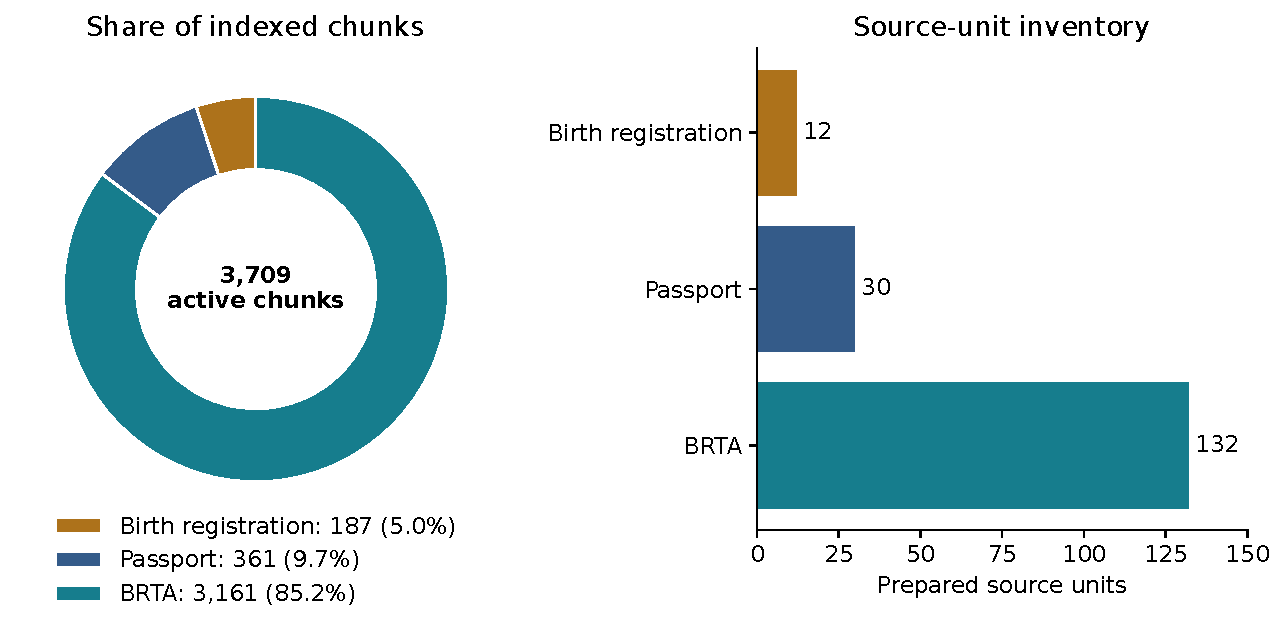
\includegraphics[width=\linewidth]{generated/corpus_distribution.pdf}
\caption{Active corpus composition from the frozen evidence manifest: 3,709 chunks and 174 prepared source units. Chunk share reflects document length and splitting, not demand, accuracy or unique facts.}\label{fig:corpus-distribution}
\end{figure}
Figure~\ref{fig:corpus-distribution} shows the corpus imbalance: BRTA accounts for 85.2\% of chunks, passport for 9.7\% and birth/death registration for 5.0\% (rounded independently). Domain-scoped retrieval prevents this corpus-size imbalance from directly mixing unrelated services in one query. It does not establish equal retrieval difficulty or equal source coverage across domains.
The table is computed from the configured JSONL files, not from unrelated candidate directories. For the older birth/death corpus, source units are counted using its source-path metadata. That count is not equated to a unique original-PDF count. Across domains, chunk counts are an indexing property rather than the number of independent facts or questions.

\begin{table}[htbp]\centering\small
\caption{Selected unresolved active-corpus flags, counted once per derivative document. These counts may overlap.}
\begin{tabularx}{\linewidth}{p{20mm}Xr}\toprule
Domain & Flag & Documents\\\midrule
Passport & no web address & 26\\
Passport & original match unresolved & 4\\
Passport & dated document review applicability & 1\\
Passport & long document check ocr & 0\\
BRTA & no web address & 109\\
BRTA & original match unresolved & 6\\
BRTA & dated document review applicability & 21\\
BRTA & long document check ocr & 8\\
\bottomrule\end{tabularx}\end{table}

Review flags count documents in the passport/BRTA registers or their associated chunk metadata, as indicated in the table. Multiple flags may apply to one document. A missing URL does not prove that a source is false, while a present URL does not prove that the derived text is correct. The flags identify where provenance and applicability need further review.

\section{Implementation of Selected Design}
\paragraph{Dense Embedding and Search.}
With encoder $f_\theta$, normalized vectors are
\begin{equation}
v_i=\frac{f_\theta(r_i)}{\|f_\theta(r_i)\|_2},\qquad
v_q=\frac{f_\theta(q)}{\|f_\theta(q)\|_2}.
\end{equation}
For unit vectors, squared Euclidean distance satisfies
\begin{equation}
\|v_q-v_i\|_2^2=2-2v_q^\top v_i.
\end{equation}
Thus distance and cosine induce the same exact ranking for normalized vectors. The index construction does not explicitly override Chroma's distance configuration; the thesis therefore does not assert that a cosine collection was manually configured. Approximate index search can differ from an exhaustive mathematical ranking.

BGE-M3 supplies the embedding model \cite{bgem3}; Chroma stores the vectors and linked documents \cite{chroma}. The implementation uses local cached model files and CPU embedding configuration. No corpus-specific gradient training occurs during this step.

\paragraph{BM25 Sparse Search.}
BM25 indexes tokens from $r_i$. Tokenization normalizes NFC, removes zero-width characters and extracts lower-case word/Bangla token sequences. The standard scoring structure is
\begin{equation}
\mathrm{BM25}(q,d)=\sum_{t\in q}\mathrm{IDF}(t)
\frac{f(t,d)(k_1+1)}{f(t,d)+k_1(1-b+b|d|/\overline L)}.
\end{equation}
Here $f(t,d)$ is term frequency, $|d|$ is token length and $\overline L$ is mean document length. The code instantiates \code{BM25Okapi} without explicit parameter overrides, so the installed library defaults determine $k_1$, $b$ and its IDF-floor behaviour \cite{bm25,rankbm25}. Lexical matching is a separate channel; it does not construct Chroma's vectors.

\paragraph{Weighted Reciprocal Rank Fusion.}
The implementation retrieves at most 20 candidates from each channel, omitting BM25 results with non-positive scores. It assigns one-based ranks and computes
\begin{equation}
S(d)=\frac{0.55\,\mathbf{1}[d\in D]}{50+r_D(d)}+
\frac{0.45\,\mathbf{1}[d\in B]}{50+r_B(d)}.
\end{equation}
A missing-channel term contributes zero. As an illustrative calculation, a chunk at dense rank 2 and BM25 rank 5 receives $0.55/52+0.45/55\approx0.01876$. This is a rank-combination value, not confidence in factual accuracy. The fused list is limited to 15 before reranking. The weights are implementation settings; this thesis does not claim they are optimal for the dataset.

\paragraph{Reranking and Domain-Specific Logic.}
The configured cross-encoder scores query/search-text pairs. If loading fails, the code can add a lexical-coverage adjustment of $0.05\,|T_q\cap T_d|/\max(|T_q|,1)$ to the incoming score. The saved primary CivicRAG candidate traces contain cross-encoder markers, establishing that the cross-encoder route was used in those records rather than merely being configured.

Birth/death-specific boosts and evidence augmentation remain part of the selected route. These are not universal learned mechanisms for passport and BRTA. This asymmetry should be disclosed when interpreting domain differences. An isolated ablation would be required to attribute an observed change to those rules.

\paragraph{Shared Reranking versus Registration-Specific Adjustments.}
The distinction is explicit in \code{src/pipeline.py}: \code{birth_death_rules} is true only for the \code{birth_death_registration} domain, and that flag is passed to the reranker's \code{domain_boosts} option. The cross-encoder itself is shared; passport and BRTA do not skip reranking. Its base score may be written as $s_{\mathrm{CE}}(q,r_i)=g_\phi(q,r_i)$, where the pretrained cross-encoder jointly processes the query and searchable passage. For a domain $d$, the implemented adjustment has the form
\begin{equation}
s_d(q,c_i)=s_{\mathrm{base}}(q,c_i)+
\mathbf{1}[d=\mathrm{birth/death}]\,\Delta_{\mathrm{registration}}(q,c_i).
\end{equation}
Here $s_{\mathrm{base}}$ is the cross-encoder score, or the documented fallback score when that model is unavailable. $\Delta_{\mathrm{registration}}$ is the sum of applicable hand-written adjustments, not a learned probability. For example, an application-process record receives an increment of 0.08 for a detected registration how-to query; additional heading conditions can further alter that score. These increments do not have a calibrated confidence interpretation.

Separately, \code{_augment_contexts} can append an existing correction-fee row for a detected date-of-birth or other data-correction query, provided its ID is not already present. It neither writes a new fact nor creates a synthetic answer. This registration-specific supplementation is different from the shared selector's compatible-family expansion, which can also operate on passport or BRTA evidence.

These rules reflect the earlier registration-focused implementation and its document-type schema. Applying the same conditions unchanged to other domains would be inappropriate: a birth-registration correction fee is not a passport or driving-licence correction fee. Equivalent domain rules were not implemented for passport and BRTA. This is an engineering asymmetry to disclose, not evidence that the extra rules are necessary or beneficial in every case. No pipeline change is made by documenting it.

\paragraph{Applicability Selection and Context Budget.}
The selector introduced after P2 uses service, action, product and location vocabularies. It prefers section scope over broad document titles and can reject a passport-collection passage for an application question. It also screens heading-only fragments, handles explicitly flagged historical alternatives and expands compatible fee/checklist families.

The selector is implemented in \code{src/generation/evidence_selection.py}; it is neither a second LLM nor a human choosing passages during normal operation. It retains at most six whole chunks within 14,000 characters. A chunk that does not fit is skipped rather than silently cut. A later ordering fix groups compatible family members near the first eligible anchor before applying the budget. Saved replay on 30 candidate sets changed the selected IDs for the passport-fee question while leaving the other 29 selections unchanged. This establishes the scope of that replay, not a general accuracy improvement.

For eligible candidates, the selector's initial priority is
\begin{equation}
h(q,c_i)=3A_i+S_i+2T_i,
\end{equation}
where $A_i$ indicates an overlapping action label, $S_i$ an overlapping service label and $T_i$ a fee/document-type match. Product, location and action conflicts can exclude a candidate before ordering. Ties retain the incoming candidate order. Historical-alternative filtering, checklist handling and compatible-family grouping are additional procedural steps, so this equation alone is not the entire selection algorithm.

For the resulting ordered list, the greedy whole-chunk selection obeys
\begin{equation}
|E|\leq 6,\qquad \sum_{c_i\in E}\operatorname{len}(e_i)\leq 14{,}000.
\end{equation}
The second bound uses Python string length in characters, not tokenizer tokens. This is a budget constraint, not a globally optimized evidence set. Skipping an oversized chunk can allow a later shorter chunk to enter the prompt.

An unknown or broad query can still retain unrelated material. Lexical applicability is not entailment, and a passage may contain mixed procedures even when its heading matches. The selector's decisions and expanded IDs are therefore retained in a trace. Removing the selector remains a proposed ablation, not a completed experiment in this manuscript.

\paragraph{Answer Generation and Safety Behaviour.}
Qwen3:8b receives the normalized question and selected evidence through Ollama \cite{qwen3,ollama}. The comparison uses temperature 0.05, top-$p$ 0.9, output limit 1,200 tokens, repetition penalty 1.18, repeat window 256 and selected-route context window 8,192. Qwen3 thinking is disabled. The prompt requests evidence-grounded Bangla responses and preservation of service conditions.

The current comparison bypasses legacy controlled extraction and question-category templates. If no applicable evidence remains, it returns a clarification/insufficient-information response. A heuristic language check can replace unsuitable-language output. A length finish reason produces an explicit incomplete-output warning. These are operational safeguards, not a complete factual verifier.

The answer's Sources footer identifies supplied context IDs, not verified supporting citations for each claim. The saved \code{raw_generation} field is produced after the generator's existing response canonicalization and should not be described as untouched token-level model output. Candidate sources and actual \code{answer_contexts} are stored separately to avoid evaluating unused passages as if the model had seen them.

\paragraph{Matched Simple RAG Baseline.}
The isolated runner \path{scripts/run_simple_matched.py} performs dense-only top-six retrieval. It does not call BM25 fusion, reranking, applicability selection, sibling expansion or controlled answers. It applies the same whole-chunk character budget, selected-route generation prompt, Qwen3 settings and language/truncation handling as the comparison configuration. The \code{selected_evidence=True} generator flag chooses the shared prompt; it does not invoke the selector inside the baseline.

\begin{table}[htbp]\centering\small
\caption{Controlled and varied elements of the main comparison.}
\begin{tabularx}{\linewidth}{p{44mm}XX}\toprule
Element & Simple RAG & CivicRAG\\\midrule
Corpus and questions & Same & Same\\
Generator and prompt & Qwen3, matched & Qwen3, matched\\
Dense retrieval & Top 6 & Top 20\\
BM25 and RRF & Absent & Present\\
Reranker & Absent & Present\\
Applicability/expansion & Absent & Present\\
Final context limit & 6 / 14,000 characters & 6 / 14,000 characters\\
Controlled answer bypass & Absent & Absent\\\bottomrule
\end{tabularx}\end{table}

The comparison intentionally keeps the baseline credible. It does not weaken the generator, restrict access to the corpus or remove successful baseline answers. It measures a bundled pipeline difference and cannot independently establish the benefit of every additional component.

\chapter{Result Analysis}\section{Performance Evaluation}
\paragraph{Needs-Analysis Results: Separate from System Performance.}
The three survey exports contain 66, 13 and 7 submissions, respectively (86 total). One explicit non-consenting submission is excluded. Of the 85 affirmative-consent submissions, four report an age below 18 and two omit age. The primary analysis therefore includes 79 adult submissions. No identical complete submission was found after aligning the service blocks, but this does not establish unique participant identities. The analysis is reproducible from the private archive using \path{scripts/analyze_needs_survey.py}; public artifacts contain aggregate counts, inclusion rules and an archive hash only.

The sample is concentrated among younger adults and men: 63/79 (79.7\%) report age 18--25, and 73/79 (92.4\%) report male gender. Recruitment and invitation counts are unavailable. Findings describe this responding sample and must not be extrapolated to all Bangladeshi citizens. They are not results from the 30-question chatbot experiment.

\begin{table}[htbp]\centering\small
\caption{Needs-analysis responses among consenting adults. Denominators exclude blank answers to each item.}\label{tab:needs-survey}
\begin{tabularx}{\linewidth}{Xr}\toprule
Response & Count / valid responses (percentage)\\\midrule
Would use the proposed AI assistant & 55/77 (71.4\%)\\
Would not use it & 13/77 (16.9\%)\\
Unsure about using it & 9/77 (11.7\%)\\
Would recheck even verified information & 42/76 (55.3\%)\\
Bangla would be more comfortable & 19/77 (24.7\%)\\
Either Bangla or English acceptable & 50/77 (64.9\%)\\
Would recommend if it works well & 67/76 (88.2\%)\\
\bottomrule\end{tabularx}\end{table}

Among valid willingness responses, 55/77 (71.4\%) would use the prospective assistant, 13/77 (16.9\%) would not and 9/77 (11.7\%) were unsure. The two missing responses are not counted as either acceptance or rejection. For trust in verified information, 30/76 (39.5\%) answered yes, 4/76 (5.3\%) no and 42/76 (55.3\%) would recheck. Positive willingness and cautious trust can coexist: the questionnaire supports the need for helpful information with verification opportunities, not unrestricted reliance on AI.

Figures~\ref{fig:survey-trust} and \ref{fig:survey-features} visualize these preferences and the requested kinds of assistance.

\begin{figure}[htbp]\centering
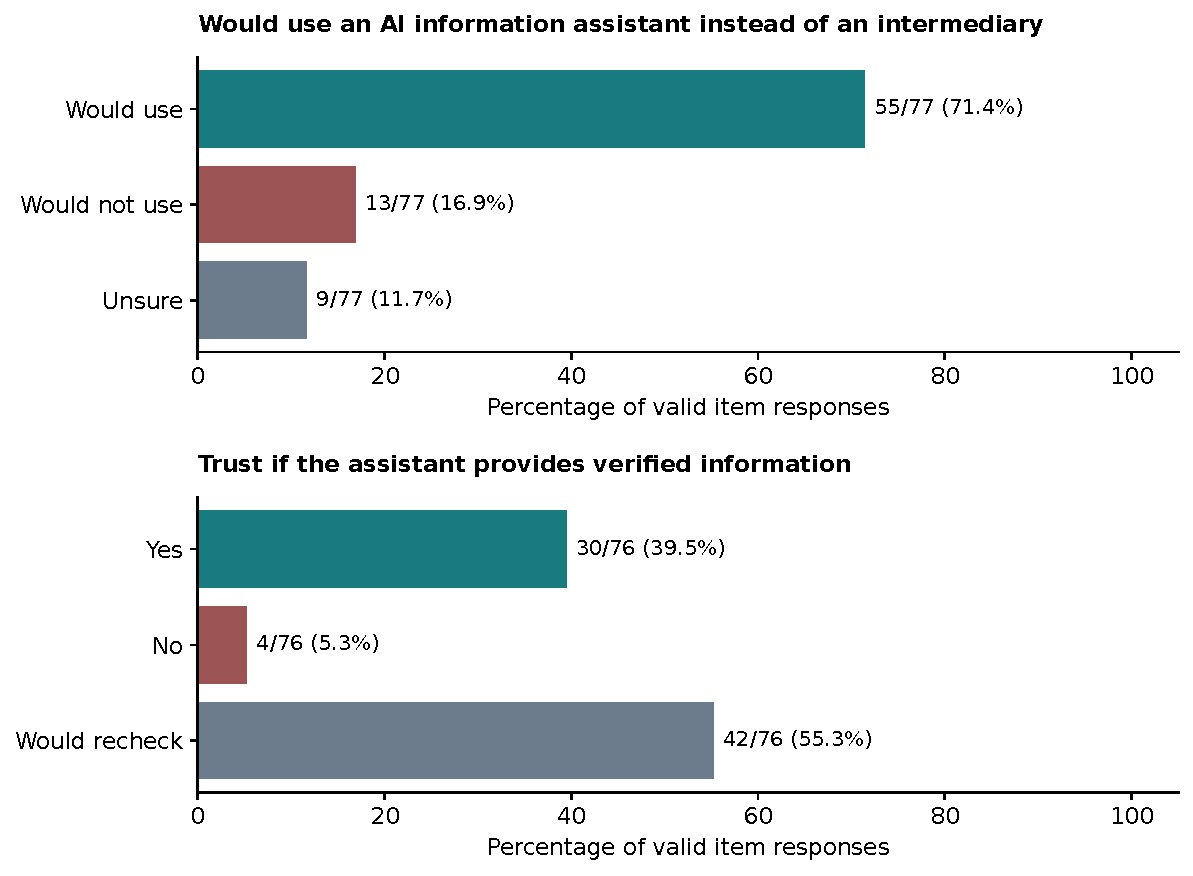
\includegraphics[width=\linewidth]{generated/survey_willingness_trust.pdf}
\caption{Stated willingness and conditional trust in the needs-analysis questionnaire. Only consenting adult submissions are included; denominators differ because of missing answers.}\label{fig:survey-trust}
\end{figure}

\begin{figure}[htbp]\centering
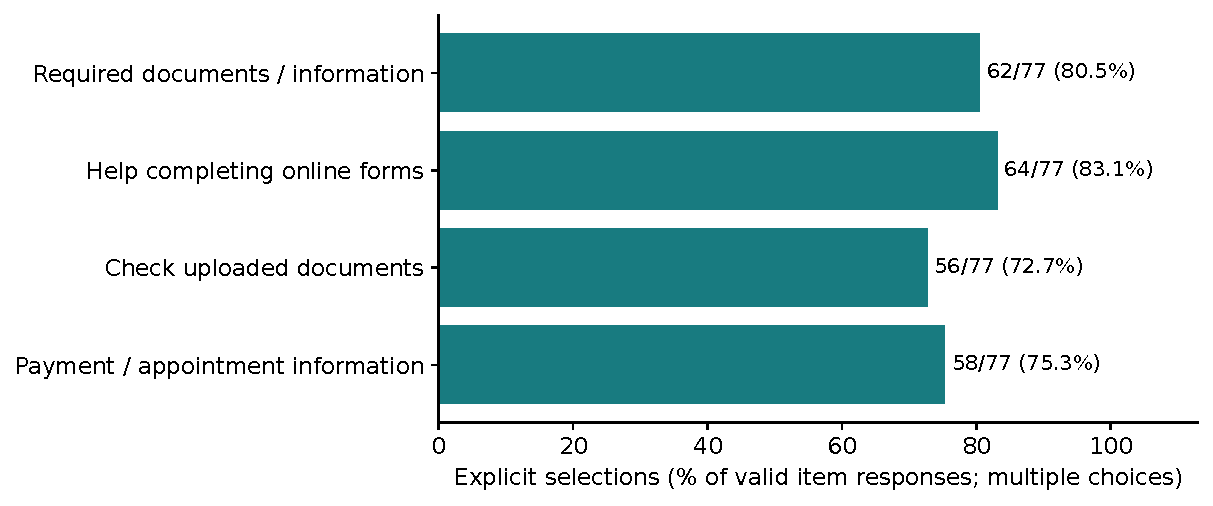
\includegraphics[width=\linewidth]{generated/survey_features.pdf}
\caption{Requested assistance, based on explicit selections among 77 valid responses. Multiple choices were allowed. One ``all options'' response is not expanded, so explicit-choice counts are conservative. Requested features are not necessarily implemented capabilities.}\label{fig:survey-features}
\end{figure}

Required-document information (80.5\%) and payment/appointment information (75.3\%) align with the implemented question-answering scope. Form-completion assistance (83.1\%) and uploaded-document checking (72.7\%) indicate additional expectations beyond that scope. This distinction prevents reporting questionnaire demand as proof that the system already satisfies every requested function.

The language item does not establish a majority preference for Bangla-only operation. Nineteen of 77 respondents (24.7\%) said Bangla would be more comfortable, 50 (64.9\%) accepted either Bangla or English and eight (10.4\%) answered no. Bangla-focused evaluation is therefore a project scope decision consistent with part of the expressed need, rather than a requirement endorsed exclusively by most respondents. Conditional recommendation was positive for 67/76 (88.2\%), but the question assumes the assistant works well; it is not satisfaction measured after using CivicRAG.

\paragraph{Experimental Design.}
The primary comparison uses the same 30 Bangla questions and domain-scoped corpus for Simple RAG and CivicRAG. Each system produced one saved answer per question using Qwen3:8b, the matched generation prompt and the same context and output limits. Simple RAG uses dense retrieval without fusion, reranking or applicability selection; CivicRAG includes these stages as described in Section 4.2. The comparison measures the combined configuration difference, not the isolated contribution of each component.

There are ten questions each for birth registration, passport and driving-licence services. All are labelled direct in the saved plan. They concern requirements, fees, time, application, correction, renewal, replacement and status. They were reused during development, so these are development-set results rather than estimates on an unseen benchmark. The source answers and hashes are preserved in the evaluation archive. No answers were regenerated for scoring or thesis preparation.

\paragraph{Operational Outcomes.}
Table~\ref{tab:operational-final} reports saved latency and context size. Both systems completed 30 requests; completion is not a correctness label.
\begin{table}[htbp]\centering\small
\caption{Operational measurements for the matched 30-question runs. Times are seconds; runs occurred separately.}\label{tab:operational-final}
\begin{tabularx}{\linewidth}{Xrr}\toprule
Measure & Simple RAG & CivicRAG\\\midrule
Completed requests & 30 & 30\\
Mean elapsed time & 193.699 & 181.823\\
Median elapsed time & 181.060 & 161.845\\
95th percentile & 319.910 & 285.100\\
Mean supplied passages & 6.000 & 4.900\\
Mean context characters & 5218.900 & 3948.033\\
Mean Bangla-letter fraction & 0.935 & 0.933\\\bottomrule
\end{tabularx}\end{table}
CivicRAG supplied fewer passages and characters on average. Its saved mean latency was also lower, but machine load, thermal conditions and initialization were not controlled across the two runs. Therefore the table does not establish a hardware-normalized speed advantage. Bangla-letter fraction measures script use after removing the source footer; it is not a fluency or correctness score.

\paragraph{Completed RAGAS and Custom Context Evaluation.}
The evaluator uses RAGAS 0.2.15 and actual supplied answer contexts, not every retrieved candidate \cite{ragas}. The official versioned metrics reference documents the metric interfaces \cite{ragas_docs}; its cited documentation snapshot is 0.2.12, whereas the recorded installed package is 0.2.15. There are $30\times2\times3=180$ completed metric scores, all valid, with no missing final scores. The appended Sources footer is removed before evaluation; response wording is otherwise preserved.

Faithfulness estimates support for the response statements in the supplied context:
\begin{equation}
F=\frac{\sum_{j=1}^{m}\mathbf{1}[a_j\text{ is supported by context}]}{m}.
\end{equation}
Here $a_j$ is a judge-extracted statement. This tests textual support, not current legal validity. Answer relevancy reconstructs three questions from a response and compares their BGE-M3 embeddings with the original question, with the metric's noncommittal-response handling. It is not similarity to a reviewed reference answer.

The third measure is a custom binary RAGAS AspectCritic. It asks whether most supplied context concerns the requested service, procedure and conditions, instructing the judge to ignore the response. Each context set receives 0 or 1. Its mean is therefore a share of positively judged context sets, not passage-level context precision or recall.

The judge is Qwen3:8b, also the answer generator. The evaluation uses temperature zero, seed 20260924, non-thinking mode, a 16,384-token context window and a 4,096-token output allowance. Stock evaluation prompts are applied to Bangla content. This completed computation remains an exploratory self-judge evaluation: a fixed seed and valid output format do not make the judge independent or its scores equivalent to factual accuracy.

Table~\ref{tab:ragas-final} presents the completed means, and Figure~\ref{fig:ragas-final} visualizes the same values.
\begin{table}[htbp]\centering\small
\caption{Completed saved-answer evaluation: Qwen3 self-judge scores, not independent accuracy.}\label{tab:ragas-final}
\begin{tabularx}{\linewidth}{Xrrrr}\toprule
Metric & Simple & CivicRAG & $\Delta$ & Pairs\\\midrule
Faithfulness & 0.7983 & 0.7323 & -0.0660 & 30\\
Answer relevancy & 0.8460 & 0.8375 & -0.0085 & 30\\
Custom context relevance & 0.9333 & 0.9667 & +0.0333 & 30\\
\bottomrule\end{tabularx}\end{table}

\begin{figure}[htbp]\centering
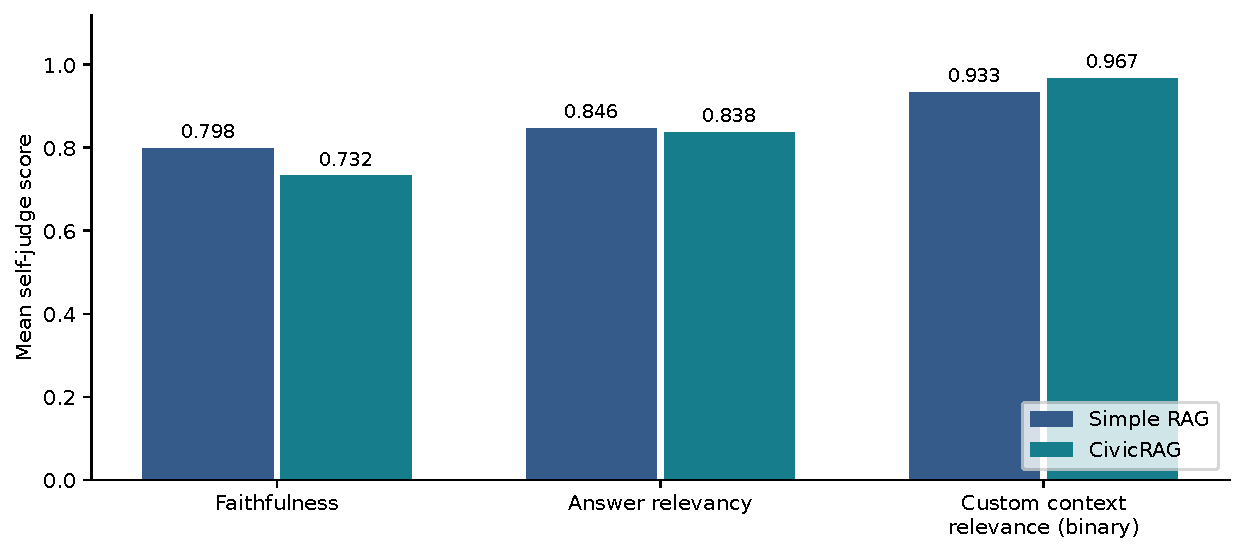
\includegraphics[width=\linewidth]{generated/ragas_final_chart.pdf}
\caption{Completed local self-judge scores for matched saved answers, with 30 valid scores per system and measure. Custom context relevance is binary and distinct from standard context precision/recall.}\label{fig:ragas-final}
\end{figure}
Simple RAG has higher mean faithfulness (0.7983 versus 0.7323) and slightly higher answer relevancy (0.8460 versus 0.8375). CivicRAG has higher custom context relevance (0.9667 versus 0.9333), corresponding to 29 versus 28 positive context-set judgments. These results describe different aspects of behaviour and do not establish a single overall winner.

\paragraph{Provisional Retrieval-Only Evaluation.}
A separate experiment compares BM25-only, dense-only and weighted Hybrid RRF on the same 30 questions before reranking, registration boosts and evidence selection. No answer generation occurs in this experiment. The top-five result union for each question forms a relevance pool; an assistant reviewed 309 question/passage pairs representing 192 unique passages. The labels are 105 relevant, 199 irrelevant and five uncertain.

These are unblinded, single-assistant labels, not independently human-verified ground truth or original-document legal verification. Four questions containing uncertain labels are excluded from all three methods, leaving 26 for Hit, Precision and MRR. One further question has no relevant passage in its judged pool; pooled Recall and nDCG therefore use 25 questions. This exclusion does not prove that the entire database lacks useful evidence.

The following equations specify the ranked-retrieval measures used in this study. Let $z_{qi}$ indicate whether the chunk at rank $i$ is labelled relevant, and let $R_q$ be the relevant IDs in the judged pool. For each eligible question:
\begin{align}
\mathrm{Precision@5}(q)&=\frac{1}{5}\sum_{i=1}^{5}z_{qi},\\
\mathrm{Hit@k}(q)&=\mathbf{1}\left[\sum_{i=1}^{k}z_{qi}>0\right],\quad k\in\{1,5\},\\
\mathrm{RR@5}(q)&=\begin{cases}1/r_q,&r_q\leq5,\\0,&\text{no relevant result in top five},\end{cases}\\
\mathrm{Recall@5}_{\mathrm{pool}}(q)&=\frac{|\mathrm{Top5}(q)\cap R_q|}{|R_q|}.
\end{align}
MRR@5 averages RR@5 over eligible questions. Recall is undefined for an empty relevant pool. Following the normalized cumulative-gain framework \cite{ndcg}, with binary relevance the discounted measure is
\begin{equation}
\mathrm{nDCG@5}_{\mathrm{pool}}(q)=
\frac{\sum_{i=1}^{5}z_{qi}/\log_2(i+1)}
{\sum_{i=1}^{\min(5,|R_q|)}1/\log_2(i+1)}.
\end{equation}
Incomplete relevance judgments can affect retrieval evaluation \cite{incompletejudgments}. Pooled Recall and nDCG use only relevant passages found in the pooled rankings, not exhaustive corpus labels. Missing retrieved positions contribute zero to Precision's fixed denominator of five. Near-duplicate IDs remain distinct scoring units.

Table~\ref{tab:retrieval-overall} gives overall results. Asterisks denote pooled, rather than corpus-wide, relevance denominators.
\begin{table}[htbp]\centering\small
\caption{Overall: provisional retrieval-only scores with assistant-reviewed labels. Hit, precision and MRR use 26 questions; pooled recall and nDCG use 25.}\label{tab:retrieval-overall}
\begin{tabularx}{\linewidth}{Xrrrrrr}\toprule
Method & H@1 & H@5 & P@5 & R@5* & MRR@5 & nDCG@5*\\\midrule
BM25 & 0.3077 & 0.6538 & 0.2769 & 0.3523 & 0.4179 & 0.3553\\
Dense & 0.6923 & 0.8846 & 0.5000 & 0.7221 & 0.7821 & 0.7156\\
Hybrid RRF & 0.4231 & 0.8846 & 0.4462 & 0.6173 & 0.6263 & 0.5863\\
\bottomrule\end{tabularx}\end{table}

Dense retrieval leads on Hit@1, Precision@5, pooled Recall@5, MRR@5 and pooled nDCG@5. Dense and Hybrid RRF tie on overall Hit@5 (0.8846). Thus adding BM25 through these fixed fusion weights does not improve every first-stage ranking measure. These provisional results neither invalidate all uses of hybrid retrieval nor prove the complete answer pipeline inferior: later reranking and selection are deliberately absent.

\section{Analysis of Design Solutions}
\paragraph{What the Diagnostics Show.}
Generation-only trials supplied manually inspected passages for three known questions, then varied evidence order and added distracting passages. Better responses with relevant-only evidence still used the LLM; they were not controlled template answers. The trials showed why context selection deserved attention, but did not establish an automatic selector's performance on arbitrary queries. This distinction is consistent with research separating retrieval quality from context use \cite{trase,lostmiddle}.

The final matched comparison tests the automatically selected evidence rather than those manually curated diagnostic contexts. The RAGAS result is mixed: more positively judged context sets coexist with lower mean faithfulness. One possible explanation is that the remaining context contains conditions the generator combines incorrectly, but the current comparison does not isolate that mechanism. A context score cannot replace inspection of the answer.

\paragraph{Illustrative Outputs Provided by the Authors.}
The following three examples were supplied with the thesis revision request. All are reported with route \code{llm_selected_evidence}. Their reported times differ from the frozen comparison rows, whose corresponding elapsed times are 204.17, 147.21 and 180.81 seconds. We therefore retain the examples as author-supplied qualitative demonstrations and do not insert their timings or wording into the aggregate benchmark. The excerpts below preserve selected supplied sentences; they are neither gold answers nor current official instructions.

For passport services, the question is \bn{পাসপোর্ট হারিয়ে গেলে কী করতে হবে?}, with a supplied time of 240.45 seconds. The response includes:
\begin{quote}
\bn{হারানো পাসপোর্টের ক্ষেত্রে অথবা চুরি হলে দ্রুত নিকটস্থ থানায় জিডি (GD) করতে হবে।}\\
\bn{পুনরায় পাসপোর্টের জন্য আবেদনের সময় পূর্ববর্তী পাসপোর্টের ফটোকপি এবং জিডি কপি সহ আবেদনপত্র দাখিল করতে হবে।}
\end{quote}
The response addresses replacement rather than unrelated passport collection. Its additional identity-document and occupation-specific requirements still need condition-by-condition verification: a useful core instruction does not make every appended requirement applicable to every applicant. The route confirms model generation after selection, not independent validation.

For birth registration, the question is \bn{জন্মনিবন্ধন অনলাইনে কীভাবে করব?}, with a supplied time of 176.82 seconds. The response directs the user to \url{https://bdris.gov.bd} and includes:
\begin{quote}
\bn{সমস্ত প্রয়োজনীয় তথ্য পূরণ করুন এবং আবেদন সাবমিট করুন।}\\
\bn{দুইটি জমজ সন্তানের ক্ষেত্রে, প্রথম সন্তানের জন্ম নিবন্ধন শেষ হওয়ার পরে দ্বিতীয় সন্তানের জন্ম নিবন্ধন করতে হবে।}
\end{quote}
The portal-oriented answer aligns with an online application question. However, the unsolicited twin-specific condition shows that source-related content can enter a general answer without being requested. This example illustrates the need to separate general steps from exceptional cases, rather than assuming additional detail is always an improvement.

For BRTA, the question is \bn{BRTA-এর ড্রাইভিং পরীক্ষায় কী কী থাকে?}, with a supplied time of 183.21 seconds. The response lists:
\begin{quote}
\bn{লিখিত পরীক্ষা}\\
\bn{মৌখিক পরীক্ষা}\\
\bn{ব্যবহারিক পরীক্ষা}
\end{quote}
The short list is more directly usable than a long legal extract. Nevertheless, the actual comparison trace discussed in Section 4.4 contains neighbouring licence topics, so this apparently clear answer is not evidence that all selected passages were applicable. Its supplied demonstration wording also differs slightly from the stored response. Across the three examples, local response latency remains substantial for interactive use.

\paragraph{Paired Answer Observations.}
Saved answers show both useful changes and regressions. Passport-document and fee answers become more task-aligned in CivicRAG, whereas the birth-registration timing response substitutes an application deadline for a processing time. Driving-licence status remains problematic. These examples explain why the evaluation retains multiple measures rather than declaring correctness from answer length or source IDs.

The authors' domain-informed preference for some more complete answers is useful qualitative feedback. Without a completed consistent review sheet, it is not converted into an aggregate expert accuracy percentage. Likewise, automatically assigned context labels cannot be relabelled as human judgments.

\section{Final Design Adjustments}
The evaluated configuration includes automatic applicability screening and the compatible-family ordering correction. Previously, compatible sibling fee sections could be appended after other candidates and then excluded by the context budget. Grouping them near the first eligible anchor changed the selected IDs for one question in a saved 30-case replay. This is a measured replay observation, not proof of general answer improvement.

The main CivicRAG answer file was generated after that correction. Its corpus, prompts and configuration were frozen for the matched comparison. No architecture change, model retraining or new answer generation was introduced while computing the reported metrics. The selected-evidence path bypasses older controlled-answer templates; the qualitative examples should not be described as those templates' output.

Documentation refinements, including birth-registration terminology and the architecture diagrams, do not alter the underlying collection identifiers, code or saved results. The label retained in stored files is a provenance identifier, not an expansion of the evaluated service scope.

\section{Statistical Analysis}
Survey percentages use valid item responses rather than a fixed denominator for every question. Unknown recruitment, demographic concentration and unverified repeat participation prevent nationally representative inference. These descriptive needs-analysis statistics are separate from the paired system results.

Statistical conclusions depend on the evaluation design and the assumptions of the selected procedure \cite{drorstats}. Our paired resampling describes uncertainty within the saved question set; it does not establish external validity. For each automatic metric, define $\delta_q=s_{\mathrm{Civic},q}-s_{\mathrm{Simple},q}$. All 30 pairs have valid scores. The saved evaluator resamples the 30 paired differences with replacement 2,000 times, using seed 20260924, and reports empirical 95\% intervals. Table~\ref{tab:ragas-intervals} reproduces those saved intervals rather than recomputing a different protocol.
\begin{table}[htbp]\centering\small
\caption{Paired CivicRAG minus Simple RAG differences with descriptive bootstrap intervals.}\label{tab:ragas-intervals}
\begin{tabularx}{\linewidth}{Xrr}\toprule
Metric & Mean $\Delta$ & 95\% interval\\\midrule
Faithfulness & -0.0660 & [-0.1787, 0.0410]\\
Answer relevancy & -0.0085 & [-0.0347, 0.0194]\\
Custom context relevance & +0.0333 & [0.0000, 0.1000]\\
\bottomrule\end{tabularx}\end{table}

The faithfulness and answer-relevancy intervals span zero; the custom binary context-relevance interval reaches zero. They reflect question resampling within this reused set, not judge calibration, repeated-generation variance or corpus representativeness. We therefore make no statistically established claim of overall factual superiority.

Per-domain retrieval results are shown in Tables~\ref{tab:retrieval-passport}--\ref{tab:retrieval-brta}. Values are question-level means over eligible questions; the overall score weights the eligible questions, not the three domain means equally.
\begin{table}[htbp]\centering\small
\caption{Passport: provisional retrieval-only scores with assistant-reviewed labels. Hit, precision and MRR use 8 questions; pooled recall and nDCG use 8.}\label{tab:retrieval-passport}
\begin{tabularx}{\linewidth}{Xrrrrrr}\toprule
Method & H@1 & H@5 & P@5 & R@5* & MRR@5 & nDCG@5*\\\midrule
BM25 & 0.5000 & 0.7500 & 0.3000 & 0.3088 & 0.5833 & 0.3798\\
Dense & 0.7500 & 1.0000 & 0.6500 & 0.7173 & 0.8750 & 0.7607\\
Hybrid RRF & 0.3750 & 1.0000 & 0.4750 & 0.5253 & 0.6562 & 0.5328\\
\bottomrule\end{tabularx}\end{table}

\begin{table}[htbp]\centering\small
\caption{Birth registration: provisional retrieval-only scores with assistant-reviewed labels. Hit, precision and MRR use 9 questions; pooled recall and nDCG use 9.}\label{tab:retrieval-birth_death_registration}
\begin{tabularx}{\linewidth}{Xrrrrrr}\toprule
Method & H@1 & H@5 & P@5 & R@5* & MRR@5 & nDCG@5*\\\midrule
BM25 & 0.3333 & 0.6667 & 0.2667 & 0.4370 & 0.4296 & 0.3938\\
Dense & 0.5556 & 0.7778 & 0.4222 & 0.6963 & 0.6481 & 0.6173\\
Hybrid RRF & 0.4444 & 0.8889 & 0.4222 & 0.6685 & 0.6148 & 0.5882\\
\bottomrule\end{tabularx}\end{table}

\begin{table}[htbp]\centering\small
\caption{BRTA: provisional retrieval-only scores with assistant-reviewed labels. Hit, precision and MRR use 9 questions; pooled recall and nDCG use 8.}\label{tab:retrieval-brta}
\begin{tabularx}{\linewidth}{Xrrrrrr}\toprule
Method & H@1 & H@5 & P@5 & R@5* & MRR@5 & nDCG@5*\\\midrule
BM25 & 0.1111 & 0.5556 & 0.2667 & 0.3006 & 0.2593 & 0.2875\\
Dense & 0.7778 & 0.8889 & 0.4444 & 0.7560 & 0.8333 & 0.7809\\
Hybrid RRF & 0.4444 & 0.7778 & 0.4444 & 0.6518 & 0.6111 & 0.6377\\
\bottomrule\end{tabularx}\end{table}

Dense and hybrid search both achieve passport Hit@5 of 1.0000 on eight eligible questions. For birth registration, hybrid Hit@5 is 0.8889 versus dense 0.7778 on nine questions, while dense retains stronger MRR. In BRTA, dense Hit@5 is 0.8889 versus hybrid 0.7778. These differences show why per-domain analysis is useful, but the small eligible samples and provisional labels limit generalization.

Uncertain questions excluded consistently across methods concern passport fees, passport renewal, birth-date proof and licence renewal. The licence-status pool contains no labelled relevant passage and is omitted only from pooled Recall/nDCG denominators. Uncertain labels are not treated as irrelevant, and missing scores are not replaced with zeros.

\paragraph{Exploratory Overnight Labeling.}
A separate Qwen3 labeling job completed 455 judgments over saved candidate and supplied passages: 176 relevant, 191 irrelevant and 88 uncertain. It hides system names, ranks and responses from the judge, but shares the generator's model family. Under its stricter requirement for complete, nonempty relevant pools, only one of 30 questions is scorable. This is a completed labeling run with incomplete adjudication, not a completed 30-question retrieval benchmark.

The single scorable passport question has Precision@5 of 0.8 for Simple RAG and 1.0 for CivicRAG, with pooled Recall@5 of 0.8 and 1.0. Those numbers cannot support a system-level conclusion. This pool differs from the three-retriever top-five pool and its labels were not merged with the assistant-reviewed study. In particular, 455 judgments and 309 judgments are not two versions of one gold dataset.

\section{Comparisons and Relationships}
The secondary model runs use the same selected-evidence configuration and matching ordered context content. Table~\ref{tab:models-final} summarizes operational outcomes; no equivalent RAGAS comparison is claimed for these secondary models.
\begin{table}[htbp]\centering\small
\caption{Secondary generator runs on the selected-evidence configuration. Language rejections are operational events, not factual error counts.}\label{tab:models-final}
\begin{tabularx}{\linewidth}{Xrrr}\toprule
Model & Requests & Mean seconds & Language rejections\\\midrule
Qwen3:8b & 30 & 181.82 & 0\\
Llama3 & 30 & 148.64 & 7\\
Qwen2.5:7b & 30 & 147.38 & 1\\\bottomrule
\end{tabularx}\end{table}
Qwen3 was a practical choice for the main comparison, not an established best model for Bangla. Its model family supports the local deployment \cite{qwen3}; the observed outcomes belong to these particular recorded runs. Language rejection does not prove a response was factually wrong, and acceptance does not prove it was correct.

The comparison has two distinct levels. The answer-pipeline experiment holds generator settings fixed and varies retrieval plus later evidence processing. The retrieval-only experiment compares ranking before those later stages. A strong first-stage dense ranking can coexist with a helpful hybrid-pipeline answer on an individual question; conversely, a positive context-set judgment can coexist with an unsupported generated statement.

The earlier 58-question registration-focused retrieval study uses different questions and labels and is not pooled into the current tables. NextRAG informs the method \cite{nextrag}, but its financial-domain scores are not benchmark competitors here. No same-dataset experiment against that external system was performed.

\section{Discussions}
The strongest established contribution is a source-traceable dataset and a working integration that permits inspection from document preparation to selected evidence and answer. The comparison also identifies concrete strengths and limitations: CivicRAG improves some task-aligned outputs and the custom context-set score, while the dense baseline has stronger mean faithfulness and several first-stage retrieval measures.

The findings do not justify abandoning evidence inspection merely because an automatic mean is high. Both a passage's applicability and the generator's interpretation matter. The automated evaluation measures text support and relevance, whereas current legal validity, completeness for an applicant and practical usability require additional review.

The completed RAGAS calculation, provisional retrieval study and exploratory labeling run should therefore remain visibly distinct. The study demonstrates implemented capabilities and reproducible measurements without claiming universal superiority, 90--95\% accuracy or readiness for unsupervised official advice. Further improvement can build on the recorded failure cases and source provenance rather than changing several components without a controlled comparison.

\chapter{Conclusion}\section{Summary of Findings}
This thesis developed Civic.ai as a locally executable RAG-based government-service information system focused on birth registration, passport and BRTA services. Its primary contribution is the preparation and organization of a source-traceable knowledge resource. The active collection contains 3,709 chunks from 174 prepared source units, with search-oriented text separated from evidence content. Combined registration documents remain in the underlying collection, but the study does not claim evaluated death-registration capability.

The implementation adapts established RAG methods \cite{lewis2020rag,nextrag}: BGE-M3 dense retrieval, BM25, weighted RRF, reranking, automatic applicability selection and local generation. It preserves the evidence supplied to the generator and records response routes and configuration information. This makes both successful answers and failures inspectable without claiming that every source-linked response is correct.

Thirty Bangla questions were answered by CivicRAG and a matched dense-only Simple RAG baseline using Qwen3:8b. All 60 requests completed. The 180 saved-answer evaluation calculations also completed, giving mixed local self-judge results: Simple RAG has higher mean faithfulness and slightly higher answer relevancy, while CivicRAG has higher custom binary context relevance. These measures demonstrate observed behaviour, not independent factual accuracy or uniform superiority.

The separate provisional retrieval comparison provides further detail. Dense retrieval leads most overall measures, while Hybrid RRF ties dense Hit@5 overall and has higher birth-registration Hit@5 on the eligible subset. These assistant-reviewed results exclude uncertain questions and use pooled relevance, not exhaustive corpus ground truth. The overnight Qwen labeling run remains exploratory because only one question is scorable under its current rules.

The needs-analysis survey supplies a different kind of evidence: 55 of 77 valid adult willingness responses (71.4\%) favoured the proposed assistant, while 42 of 76 trust responses (55.3\%) would recheck its information. This supports the design emphasis on understandable guidance and source inspection, without demonstrating adoption or population-wide social impact.

\section{Contributions to the Field}
The principal contribution is dataset development. We organized heterogeneous civic-service materials into domain-specific retrieval records, retained original-to-derivative relationships, and preserved available metadata, URLs and unresolved review flags. This resource supports systematic investigation of civic questions rather than relying on a general model's untraceable knowledge.

The second contribution is the developed system integration. Search aliases support retrieval without becoming answer facts; chunk identifiers connect vector results to source content; and selection traces make post-retrieval decisions visible. The architecture adapts established techniques to the language and procedure distinctions of the collected documents rather than claiming a new foundation model or general-purpose RAG algorithm.

The third contribution is an auditable evaluation record. Matched baseline answers, selected contexts, model settings, local judge scores and provisional retrieval labels are retained separately. Manually selected diagnostics are not confused with automatic operation, and completed computations are not confused with validated ground truth. This separation allows future work to test specific changes without losing the current comparison.

\section{Recommendations for Future Work}
The first priority is independent, evidence-backed annotation of unseen questions and relevant passages. The set should cover paraphrases, conditional scenarios, ambiguous questions and insufficient-evidence cases across the three studied domains. Additional services, including death registration, would require explicit scope definition and evaluation rather than assuming that their appearance in a combined source proves support.

Data review should address unresolved original matches, outdated instructions, conflicting conditions and long legal OCR. Reviewed changes should be versioned with the corpus and rebuilt indexes. Relevance annotation and verification against current official documents serve different purposes and should be recorded separately.

Architectural improvements should use single-factor comparisons. Selector-on versus selector-off, adjusted context budgets and dense retrieval followed by reranking are useful candidates. Stronger multilingual generators or independent evaluation models may improve particular stages, but their benefits should be measured rather than inferred from model size or a persuasive demonstration. More capable hardware and measured runtime profiling could address the recorded interactive latency.

Finally, a prospective user study could measure clarity, usefulness and the effort needed to verify responses. Such evidence would be needed to substantiate the intended social outcomes described in the preserved Abstract. Civic.ai is presented as a developed and evaluated information system with a documented dataset contribution and bounded findings, not an official decision-making service.

\bibliographystyle{IEEEtran}\bibliography{bibliography/references}
\appendix
\chapter{Reproducibility and Evaluation Questions}This appendix retains the title in the official template and describes the build requirements for this manuscript. The source uses XeTeX-compatible Unicode fonts. The verified local build uses Tectonic, which handles compilation passes and bibliography processing.

\begin{enumerate}
\item Install a compatible TeX toolchain. This manuscript was verified with Tectonic; XeLaTeX with BibTeX is an alternative.
\item Ensure Times New Roman and Kohinoor Bangla are available. If replacement fonts are necessary, change only the font declarations in \code{main.tex} and recheck all pages. The Abstract text must remain unchanged.
\item Keep \code{core}, \code{chapters}, \code{appendix}, \code{bibliography} and \code{generated} beside \code{main.tex}.
\item From the manuscript directory run \code{tectonic --keep-logs --keep-intermediates main.tex}.
\item Review the PDF, contents pages, equations and tables. Resolve missing characters, undefined references and overflowing text before submission.
\end{enumerate}

The generated tables are included in the source package. Rebuilding the PDF does not require running the chatbot or downloading language models. Updating experimental results is a separate operation: the repository audit script reads saved artifacts and checks their configuration hashes before regenerating tables.

\chapter{Completion and Verification Requirements}The original template's appendix title is retained. The manuscript is stored with its \LaTeX\ source, bibliography and generated tables in the project repository. Git provides revision history and rollback points; the PDF is a compiled output rather than a substitute for editable source.

For hosted editing, transfer the source package while preserving its directories, select \code{main.tex} as the main document and use a Unicode-compatible compiler. Local fonts may not be available in the hosted environment. Use legally available fonts and review any layout changes. This manuscript has been compiled locally; a successful hosted build is not claimed.

Before revising the report, preserve the current Git revision. Keep manuscript edits separate from evaluation artifacts so that a reporting change does not silently alter an experiment. Compile and review the PDF before committing its source and output together. Keep incomplete scores distinct from completed results and never overwrite the unchanged Abstract while merging revisions.

Additional reproducibility notes, evaluation questions and completion requirements remain in the accompanying source package and repository. They are supporting artifacts, not replacement appendix titles or added entries in the official template's chapter index.

\end{document}
